\chapter{ML}

\section{Artificial neuron}

Artificial neurons, also called perceptrons were developed in the late 1950s and early 1960s, firstly introduced by Rosenblatt in his paper \textbf{TODO}\footnote{\url{http://citeseerx.ist.psu.edu/viewdoc/download?doi=10.1.1.335.3398&rep=rep1&type=pdf}}. His idea was to develop a model capable of simulating the activities present in the human brain cell, in order to create artificial intelligence. As it turned out, simulating the brain using such a simple model as the perceptron is impossible. However, later research discovered a considerable potential in the field of classification and regression, which lead to design of modern artificial neural networks as we know it today.

Perceptron is a simple probabilistic model, which takes several weighted real inputs and produces one real output.

\vspace{3mm}

\begin{minipage}[c]{0.35\textwidth}
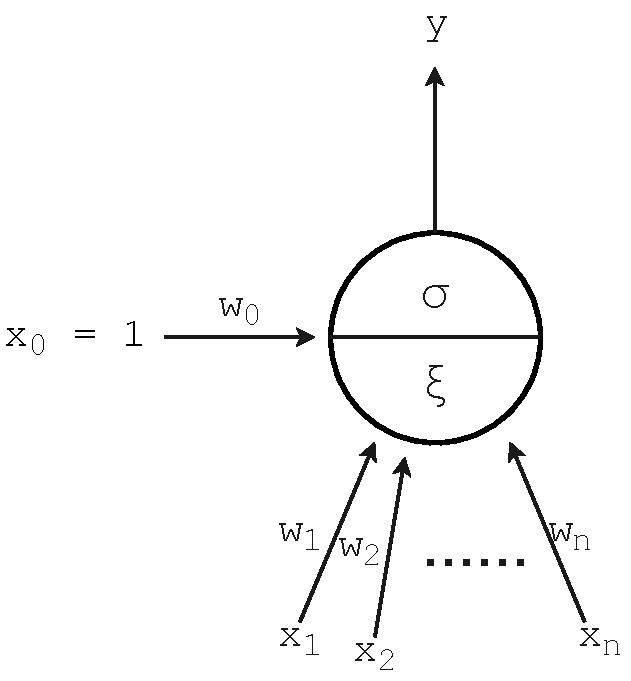
\includegraphics[width=\textwidth]{tex/images/perceptron}
\end{minipage}
\hfill
\begin{minipage}[c]{0.55\textwidth}


\begin{itemize}

\item \textbf{TODO} <---- figure caption 
\item $x_1, \cdots, x_n$ are real \textbf{inputs}
\item $x_0$ is always equal to 1
\item $w_0, w_1, \cdots, w_n$ are real \textbf{weights}
\item $\xi$ is inner \textbf{potential}, \\$\xi = w_0 + \Sigma_{i=1}^n w_i x_i$
\item $y$ is real \textbf{output} given as $y = \sigma(\xi)$
\item $\sigma$ is an \textbf{activation function}

\end{itemize}
\end{minipage}

\section{activation}
\section{loss}
\section{gradient descend + backprop}
\section{ANN}
\section{FeedForward}
\section{DeepNN}



